
\documentclass[11pt]{informatics-report}
\usepackage{color}
\usepackage{float}
\usepackage[utf8]{inputenc}
\usepackage{graphicx}
\usepackage{amsmath}
\usepackage{pdfpages}
\usepackage{hyperref}
\usepackage{pdflscape}
\usepackage[paper=A4,pagesize]{typearea}
\usepackage{subcaption}
\usepackage[square,sort,comma,numbers]{natbib} %References
\usepackage{afterpage}
\usepackage{titling}




%%%%%%%%%%%%%%%%%%%%%%%%%%%%%%%%%
% Front Matter - project title, name, supervisor name and date
%%%%%%%%%%%%%%%%%%%%%%%%%%%%%%%%%
\title{7CCSMGPR GROUP PROJECT:\\\vspace{0.2cm}Initial Report}
\author{Marcell Sarosi, }
\studentID{1542196}


\date{\today}

\abstractFile{FrontMatter/abstract.tex}

\begin{document}
\createFrontMatter
\onehalfspacing
\tableofcontents
\doublespacing

%%%%%%%%%%%%%%%%%%%%%%%%%%%%%%%%%
% Report Content
%%%%%%%%%%%%%%%%%%%%%%%%%%%%%%%%%
% You can write each chapter directly here or in a separate .tex file and use the include command.

\chapter{Project Description}

The main aim for this project is to develop a multi-host file synchroniser. To achieve this main goal, we have split the construction of this project into smaller aims that are more achievable for one person, which we will then combine to give us the end product of a file synchroniser. Although these have been split and assigned to each member we will still collaborate within the sub-tasks to ensure the quality and consistency of our code, more on this in ‘Project Organisation’.  When it came to plan our project, we decided to adopt a waterfall approach with scope to change when we advance to the next section, this was dependant on how each member was progressing after initial research into their sub-task. This means we also have an agile plan that will change as we progress through the tasks. The mobile application is being made with Android Java in Android Studio and the front end of the web application is being made with HTML, CSS and Javascript with the back end being created with PHP framework Laravel, our database is being hosted on a Digital Ocean server.

The first decision we made regarding our strategy was whether we wanted the client to have a version of the file located on their own computer where they would then edit this file then re-upload into the database. The other option was to just edit the file directly in the database with a synchronisation to be ran every X minutes, so the file on the database was up to date. We decided that the best option for our group was to hold a version locally, this was because storing locally requires less connection with the server meaning that if the client doesn’t have an Internet connection there will be no errors occurring when work is being done on the document. This also means that if the were no connection to the internet and for any reason the clients desktop shut down without an upload occurring, all the work they had completed would be lost. Our method of storing locally means that less data is required to be sent across the network, freeing up bandwidth for the client to use for other tasks. 

The next strategic decision we made was if there was a conflict of two files uploading at the same time, we decided it was best if this was handled as a server operation. As we will have access levels the priority will be given to the highest access level with the file from the lower level having to be renamed with “‘username’–updated” placed after, with a timestamp so it is clear when the file was last updated. 

As previously mentioned we broke our project down into sub-tasks, these tasks also carried a weighting depending on how important they were to the core functionality of the system. At the top level of priority are the \textbf{client-side UIs}  for the Android application and the web service, these will be the screens that provide interface functionality with the server and will consist of:

\begin{itemize}
\item -	Login Screen- Simple page to enter user details and log into the service
\item -	Register Screen - Form to get data from new users.
\item -	Directory Screen - Page listing the files on the sever and providing basic information about them to the server. This screen also facilitates downloading files.
\item -	Upload Screen - Page where the user can browse files from the phone’s memory and send them to the server.
\item -	Account Management Screen - Page where the user can view and edit their details
\end{itemize}

Also with very high priority are the server-side methods called by user action: 

\begin{itemize}
\item \textbf{Listing available files} – Retrieving basic file information from server and show to user 
\item \textbf{Downloading files} – Server sends requested file to user
\item \textbf{Uploading files } User sends file to sever
\end{itemize}

At the next level of priority, we have the functions that deal with conflict: 

\begin{itemize}
\item \textbf{Renaming File } – Facilitate functionality of renaming files on server
\item Method called by server action  \textbf{Error Handling } – Handle any faults in the upload or download process, corrupted files and incomplete messages.
\end{itemize}

Below this level of priority, we have:

\begin{itemize}
\item \textbf{Register} -  Adding user to database by generating access token, encryption, store details, setting privilege level.
\item \textbf{Authentication} – Allowing only authorised users into applicationr
\end{itemize}

Then on the lowest layer of priority are the methods:

\begin{itemize}
\item \textbf{Adjusting Privilege } -  Increase or decrease user access level
\item \textbf{Notify } – Notifying user of successful upload
\end{itemize}

Currently in our database we have four tables ready on the server. These are going to be use for holding information about; \textbf{user authentication, files in the database, version history and logging any changes}

\begin{minipage}{0.9\linewidth}
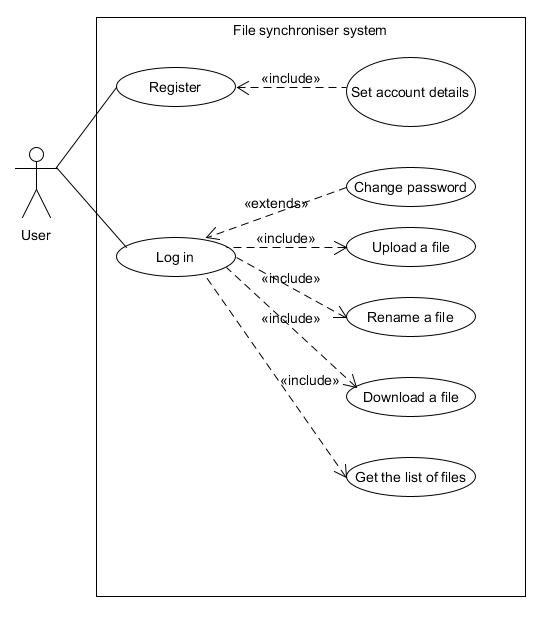
\includegraphics[width=\textwidth,height=\textheight,keepaspectratio]{Informatics_Final_Report_Template/usecase.png}
\captionof{figure}{Use Case Diagram}
\end{minipage}%

\begin{minipage}{0.9\linewidth}
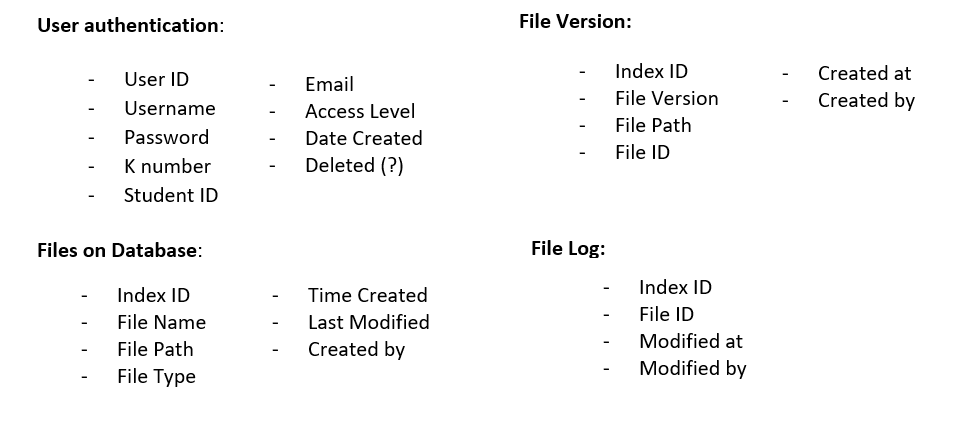
\includegraphics[width=\textwidth,height=\textheight,keepaspectratio]{Informatics_Final_Report_Template/log.PNG}
\captionof{figure}{Database Outline}
\end{minipage}%



\chapter{Project Organisation}

Working as a team is one of the most important aspects of group work, having to understand people’s strengths and boundaries can be challenging at times but communication is an important tool to use in smoothing out any wrinkles that can occur whilst working with a group of new colleagues. Within our group we have decided to have weekly meetings to discuss our current progress and allow people to air any concerns they have with their own work, giving them the opportunity to hear praise for the work so far and input from the other 5 members on anything they could be struggling with. Also, these meeting allow us to contemplate the timetable and make adjustments for the week ahead, should anyone need help.
During our initial meeting we quickly got onto discussing the roles which we thought we were most suited to, allowing us to utilise the experience we had gained from previous projects, build on any work that had already been started and talked about the areas in which people wanted to develop their skills. Marcell was very keen to take control of the mobile application as he had done a large amount of mobile development in the past and we all agreed that it was best if he led that part of the project. Coming into the first meeting Zack had already started looking at possible servers that we could use to host the database, so Zack was then elected to be the leader of any server problems we had. Yixin took the initiative during the first 48 hours and set up our GitHub repository, in doing so learnt about how GitHub processes worked, meaning she was happy to be the team member who assisted with any problems in that department. As well as these roles, Zack and Yixin are also helping the programming of the web application alongside Zihao, Trisha and Tom.
The main tool we are using for collaboration is the GitHub repository set up by Yixin, this allow us to keep track of the master copy of the file whilst also allowing each individual user to take the latest version and work on their part of the project without affecting our colleagues work. We have also got a Facebook Messenger chat, in which we have currently been organising meetings and have been discussing the functionality and the limits for our file synchroniser. Facebook Messenger also allows us the function of voting, which we have utilised already in deciding what day and time to hold our weekly meetings.
For the peer assessment we have decided to split the 100 marks equally between us all. As we are all happy with the plan and allocation of roles it seems fair that we all achieve the same weighting. Within the group we have also agreed that if anyone is struggling with their own task we will all try to help that person, meaning there is a good ‘give and take’ relationship between us all.  If there is any conflict within the group we will let each of the people explain their side of the conflict and then decide as a group the best course of action from that point, this may be siding with one person or coming up with a compromise that the group sees fit and will greater benefit the group. 

Timetable:

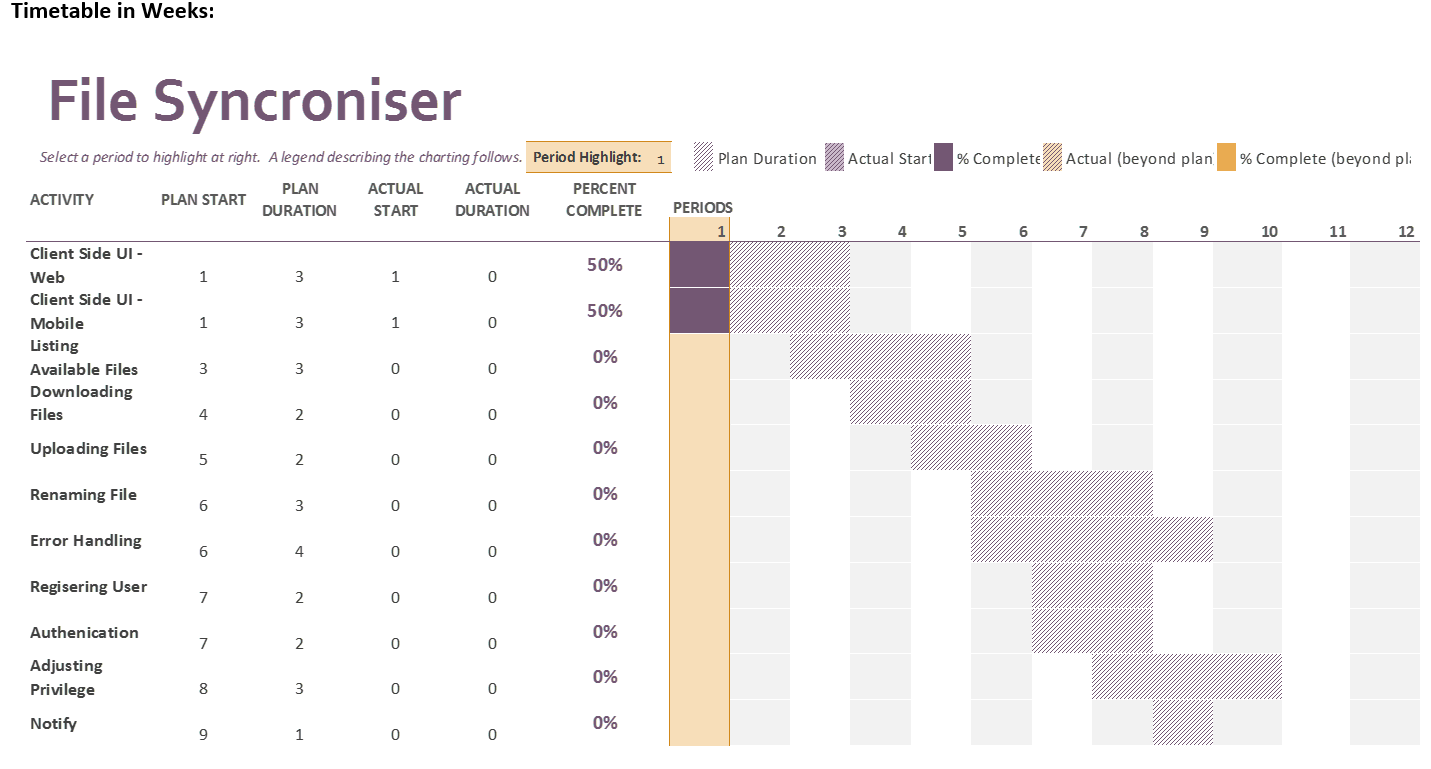
\includegraphics[angle=90, width=\textwidth,height=\textheight,keepaspectratio]{timetable}


%%%%%%%%%%%%%%%%%%%%%%%%%%%%%%%%%
% Appendices
%%%%%%%%%%%%%%%%%%%%%%%%%%%%%%%%%
\end{document}
